\documentclass[12pt,a4paper]{article}
\usepackage{amsmath,amscd,amsbsy,amssymb,latexsym,url,bm,amsthm}
\usepackage{epsfig,graphicx,subfigure}
\usepackage{enumitem,balance}
\usepackage{wrapfig}
\usepackage{mathrsfs,euscript}
\usepackage[usenames]{xcolor}
\usepackage{hyperref}
\usepackage[vlined,ruled,linesnumbered]{algorithm2e}
\usepackage{float}
\hypersetup{colorlinks=true,linkcolor=black}

\newtheorem{theorem}{Theorem}
\newtheorem{lemma}[theorem]{Lemma}
\newtheorem{proposition}[theorem]{Proposition}
\newtheorem{corollary}[theorem]{Corollary}
\newtheorem{exercise}{Exercise}
\newtheorem*{solution}{Solution}
\newtheorem{definition}{Definition}
\theoremstyle{definition}

\renewcommand{\thefootnote}{\fnsymbol{footnote}}

\newcommand{\postscript}[2]
{\setlength{\epsfxsize}{#2\hsize}
	\centerline{\epsfbox{#1}}}

\renewcommand{\baselinestretch}{1.0}

\setlength{\oddsidemargin}{-0.365in}
\setlength{\evensidemargin}{-0.365in}
\setlength{\topmargin}{-0.3in}
\setlength{\headheight}{0in}
\setlength{\headsep}{0in}
\setlength{\textheight}{10.1in}
\setlength{\textwidth}{7in}
\makeatletter \renewenvironment{proof}[1][Proof] {\par\pushQED{\qed}\normalfont\topsep6\p@\@plus6\p@\relax\trivlist\item[\hskip\labelsep\bfseries#1\@addpunct{.}]\ignorespaces}{\popQED\endtrivlist\@endpefalse} \makeatother
\makeatletter
\renewenvironment{solution}[1][Solution] {\par\pushQED{\qed}\normalfont\topsep6\p@\@plus6\p@\relax\trivlist\item[\hskip\labelsep\bfseries#1\@addpunct{.}]\ignorespaces}{\popQED\endtrivlist\@endpefalse} \makeatother

\usepackage{tikz}
\usepackage{caption}
\usepackage{listings}
% listings
\definecolor{grey}{rgb}{0.8,0.8,0.8}
\definecolor{darkgreen}{rgb}{0,0.3,0}
\definecolor{darkblue}{rgb}{0,0,0.3}
\lstset{%
    numbers=left, %行号
    numberstyle=\tiny\color{grey},
    showstringspaces=false,
    showspaces=false,%
    tabsize=4,%
    frame=shadowbox,%
    basicstyle={\ttfamily\scriptsize},%
    keywordstyle=\color{blue!80!black}\bfseries,%
    identifierstyle=,%
    commentstyle=\color{green!50!blue}\itshape,%
    stringstyle=\color{green!50!black},%
    rulesepcolor=\color{gray!20!white},
    breaklines,
    columns=flexible,
    extendedchars=false,
    %mathescape=true,
}
\providecommand{\code}[2]{\lstinputlisting[language=#2,caption=\href{run:#1}{\ttfamily #1}]{#1}}
\providecommand{\img}[1]{\includegraphics[width=0.88\textwidth]{#1}}
\usepackage{tcolorbox}
\usepackage{array}

\begin{document}
	\noindent
	
	%========================================================================
	\noindent\framebox[\linewidth]{\shortstack[c]{
			\Large{\textbf{Lab05-DynamicProgramming}}\vspace{1mm}\\
			CS214-Algorithm and Complexity, Xiaofeng Gao, Spring 2021.}}
	\begin{center}
		\footnotesize{\color{red}$*$ If there is any problem, please contact TA Haolin Zhou.}
		
		% Please write down your name, student id and email.
		\footnotesize{\color{blue}$*$ Name: Zilong Li \quad Student ID: 518070910095 \quad Email: logcreative-lzl@sjtu.edu.cn}
		
	\end{center}
	
	\begin{enumerate}
		\item \textit{Optimal Binary Search Tree.} Given a sorted sequence $K=\left \langle k_{1}, k_{2}, \ldots, k_{n} \right \rangle$ of $n$ distinct keys, and we wish to build a binary search tree from these keys. For each key $k_{i}$, we have a probability $p_{i}$ that a search will be for $k_{i}$. Some searches may be for values not in $K,$ and so we also have $n+1$ \emph{dummy keys} $d_{0}, d_{1}, d_{2}, \ldots, d_{n}$ representing values not in $K$. In particular, $d_{0}$ represents all values less than $k_{1}$, and $d_{n}$ represents all values greater than $k_{n}$. For $i=1,2, \ldots, n-1,$ the dummy key $d_{i}$ represents all values between $k_{i}$ and $k_{i+1}$. For each dummy key $d_{i}$, we have a probability $q_{i}$ that a search will correspond to $d_{i}$. Each key $k_{i}$ is an internal node, and each dummy key $d_{i}$ is a leaf. Every search is either successful (finding some key $k_{i}$ ) or unsuccessful (finding some dummy key $d_{i}$ ), and so we have $ \sum_{i=1}^{n} p_{i}+\sum_{i=0}^{n} q_{i}=1 $. 
		\begin{enumerate}
			\item Prove that if an optimal binary search tree $T$ ($ T $ has the smallest expected search cost) has a subtree $T^{\prime}$ containing keys $k_{i}, \ldots, k_{j},$ then this subtree $T^{\prime}$ must be optimal as well for the subproblem with keys $k_{i}, \ldots, k_{j}$ and dummy keys $d_{i-1}, \ldots, d_{j}$. 
			\item We define $e[i, j]$ as the expected cost of searching an optimal binary search tree containing the keys $k_{i}, \ldots, k_{j} .$ Our goal is to compute $e[1, n]$. Write the state transition equation and pseudocode using \textbf{dynamic programming} to find
			the minimum expected cost of a search in a given binary tree. (\textbf{Remark}: You may use $ w[i, j]=\sum_{l=i}^{j} p_{l}+\sum_{l=i-1}^{j} q_{l} $).
			\item Implement your proposed algorithm in C/C++ and analyze the time complexity. ({\color{blue}The framework Code-OBST.cpp is attached on the course webpage}). Give the minimum search cost calculated by your algorithm. The test case is given as following:
			\begin{table}[H]
				\setlength{\abovecaptionskip}{0cm}
				\setlength{\belowcaptionskip}{0.1cm}
				\centering		
				\begin{tabular}{|c|cccccccc|}
					\hline
					$ i $&0&1&2&3&4&5&6&7\\
					\hline
					$ p_{i} $&&0.04&0.06&0.08&0.02&0.10&0.12&0.14\\
					\hline
					$ q_{i} $&0.06&0.06&0.06&0.06&0.05&0.05&0.05&0.05\\
					\hline
				\end{tabular}
			\end{table}
			\item Please draw the structure of the optimal binary search tree in the test case, and explain the drawing process.   
		\end{enumerate}
		
		\begin{enumerate}
			\item \begin{proof}
			\textbf{Prove by contradiction.} Suppose this subtree $T^\prime$ is not optimal, then there exists a subtree $T^{\prime\prime}$ is better than $T^\prime$ on expected search cost with keys $k_i,\cdots,k_j$ and dummy keys $d_{i-1},\cdots,d_j$. Then the expeceted search cost between the two subtrees has the following relationship:
			\begin{equation}\label{eq:opt}
				e^{\prime\prime}<e^\prime
			\end{equation}
			Assume the summation of the probability on the subtree is $P$. And The summation of search cost in the remaining part is $C$. Then the Eq. \eqref{eq:opt} follows:
			\begin{equation*}
				e^{\prime\prime}P+C<e^\prime P+C
			\end{equation*}
			which means that if $T^\prime$ is replaced by the optimal subtree $T^{\prime\prime}$, a better binary search tree could be contructed than $T$. The contradiction over the optimal of the original binary search tree shows that the subtree $T^\prime$ is optimal.
			\end{proof}
			\item \begin{solution} 
			
			Consider the root of the optimal binary search tree containing keys $k_i,\cdots,k_j$. If the root is $k_r(i\leq r\leq j)$, then according to the previous subproblem, the left subtree containing $k_i,\cdots,k_{r-1}$ and the right subtree containing $k_{r+1},\cdots, k_j$ are also the optimal binary search tree.

			If $j=i-1$, the subtree only has one dummy key $d_{i-1}$, and the expected search cost is $e[i,i-1]=q_{i-1}$.

			If $j\geq i$, because once one tree become a child, the search cost for every node will be increased by 1 and the expected cost could be increased by the summation of probability in the subtree. Then the expected search cost could be calculated recursively by calculating for every $i\leq r\leq j$:
			\begin{align*}
				e[i,j] &= p_r + (e[i,r-1]+w[i,r-1])+(e[r+1,j]+w[r+1,j])\\
				&=e[i,r-1]+e[r+1,j]+w[i,j]
			\end{align*}

			As a result, the state transition equation could be stated as follows:
			\begin{equation*}
				e[i,j]=\left\{\begin{aligned}
					&q_{i-1},&&j = i-1,\\
					&\min_{i\leq r\leq j} e[i,r-1]+e[r+1,j]+w[i,j],&&j\geq i
				\end{aligned}\right.
			\end{equation*}

			The algorithm is shown in Alg. \ref{alg:opt} and function \texttt{getExpectedCost}($i$,$j$).

			\begin{function}[h]
				\caption{getExpectedCost($i$,$j$)}
				\KwData{start $i$, end $j$}
				\KwOut{the expected cost $e[i,j]$}
				\BlankLine
				\lIf(){$e[i,j]$ is initialized}{\Return{$e[i,j]$}}
				$r_{\text{min}}\leftarrow i, e_{\text{min}}\leftarrow \infty$\;
				\For(){$r\leftarrow i$ to $j$}{
					$e^\prime\leftarrow$ \getExpectedCost($i$,$r-1$) + \getExpectedCost($r+1,j$)+$w[i,j]$\;
					\If{$e^\prime\leq e_{\text{min}}$}{
						$r_{\text{min}}\leftarrow r$\;
						$e_{\text{min}}\leftarrow e^\prime$\;
					}
				}
				$root[i,j]\leftarrow r_\text{min},e[i,j]\leftarrow e_\text{min}$\;
				\Return{$e_\text{min}$}\;
			\end{function}
			\begin{algorithm}[h]
				\caption{Find the optimal binary search tree}
				\label{alg:opt}
				\KwIn{key probability $\{p_i\}_{i=1}^n$, dummy key probability $\{q_i\}_{i=0}^n$, input size $n$}
				\KwOut{expected cost $e[1,n]$}
				\BlankLine
				Initialize $w[i,j]=\sum_{l=i}^jp_l+\sum_{l=i-1}^jq_l$\;
				Initialize $e[i,i-1]=q_j$\;
				Initialize $root[i,i-1]=i-1$\;
				\getExpectedCost(1,$n$)
			\end{algorithm}
			% For the optimal binary search tree $T[i+1,j-1]$, consider inserting leftmost new nodes $k_i$/$d_{i-1}$ shown in Figure \ref{fig:lmi}. The new nodes could be either the child or the parent, depending on the overall cost.
				
			% \begin{figure}[H]
			% 	\centering
			% 	\subfigure[as a child]{\input{img/i.tex}}\hspace{3em}
			% 	\subfigure[as a parent]{\input{img/ip.tex}}
			% 	\caption{Insert the new node for the leftmost item}\label{fig:lmi}
			% \end{figure}

			% Assume $k_{i+1}$ is of cost $a_{i+1}$ in the original optimal binary search tree. And similar to the definition of $e[i,j]$, define the expected cost of the original subtree $T_L$ with the root of $k_{i+1}$ as:
			% \begin{equation*}
			% 	e_L = \frac{a_{k+1}p_{k+1}+(a_{k+1}+1)q_i+C}{\sum p_l + \sum q_l}
			% \end{equation*}
			% where $\sum$ sum up the nodes in the domain and $C$ is the overall cost of the right branch in the left subtree. Then calculate the expected cost of new subtree in both scenarios.
			% \begin{description}
			% 	\item[Case (a): as a child.]
			% 	\begin{align*}
			% 		e_{La} &= \frac{a_{k+1}p_{k+1}+(a_{k+1}+2)q_{i}+(a_{k+1}+1)p_{i}+(a_{k+1}+2)q_{i-1}+C}{\sum p_l + \sum q_l + p_i + q_{i-1}}\\
			% 		&=\frac{e_L (\sum p_l + \sum q_l)+q_i+(a_{k+1}+1)p_{i}+(a_{k+1}+2)q_{i-1}}{\sum p_l + \sum q_l + p_i + q_{i-1}}
			% 	\end{align*} 
			% 	\item[Case (b): as a parent.]
			% 	\begin{align*}
			% 		e_{Lb} &= \frac{a_{k+1}p_i+(a_{k+1}+1)q_{i-1}+(e_L+1)(\sum p_l + \sum q_l)}{\sum p_l + \sum q_l + p_i + q_{i-1}}
			% 	\end{align*} 
			% \end{description}
			% \begin{figure}[H]
			% 	\centering
			% 	\subfigure[as a child]{\input{img/j.tex}}\hspace{3em}
			% 	\subfigure[as a parent]{\input{img/jp.tex}}
			% 	\caption{Insert the new node for the rightmost item}
			% \end{figure}
			\end{solution}
			\item The implementation is as follows:
			\code{Code-OBST.cpp}{c++}

			The time complexity is analyzed as follows:
			\begin{description}
				\item[Initialization.] The initalization of $w,e,root$ costs $O(n^2)$.
				\item[Calculation.] The recurrence of the time complexity is:
				\begin{align*}
					T[i,i-1] &= O(1)\\
					T[i,j] &= \sum_{i\leq r\leq j}(T[i,r-1] + T[r+1,j] + O(1))
				\end{align*} 

				A recurrence tree could be drawn in Figure \ref{fig:tc}. The diagonal is first calculated and every step in the figure is $O(1)$.
				\begin{figure}[h]
					\centering
					\usetikzlibrary{math}
\begin{tikzpicture}
\tikzstyle{dot}=[draw,circle,fill=white,scale=0.6];
\foreach \x in {1,...,7}{
	\foreach \y in {\x,...,7}{
		\draw (\x,\y-1)--(\x,\y);
		\draw (\x+1,\y)--(\x,\y);
	}
}

\foreach \x in {1,...,8}{
	\pgfmathparse{int(\x-1)}
	\foreach \y in {\pgfmathresult,...,7}{
		\node[dot] at (\x,\y) {\x,\y};
	}
}
\end{tikzpicture}

					\caption{Time Complexity Analysis}
					\label{fig:tc}
				\end{figure}

				So, the time complexity is $(n^2+n)/2 = O(n^2)$.
			\end{description}
			As a result, the time complexity comes to $O(n^2)$.

			And the running result is:
			\begin{tcolorbox}
The cost of the optimal binary search tree is: 3.12
			\end{tcolorbox}

			\item The continued running result is:
			\begin{tcolorbox}
The structure of the optimal binary search tree is:\\
k5 is the root\\
k2 is the left child of k5\\
k1 is the left child of k2\\
d0 is the left child of k1\\
d1 is the right child of k1\\
k3 is the right child of k2\\
d2 is the left child of k3\\
k4 is the right child of k3\\
d3 is the left child of k4\\
d4 is the right child of k4\\
k7 is the right child of k5\\
k6 is the left child of k7\\
d5 is the left child of k6\\
d6 is the right child of k6\\
d7 is the right child of k7
			\end{tcolorbox}

			According to the output, the binary search tree could be drawn in Fig. \ref{fig:bst}.

			\begin{figure}[h]
				\centering
				\begin{tikzpicture}[scale=0.7,every node/.style={scale=0.7}]
\tikzstyle{tnode}=[circle,draw,minimum width=0.5cm];
\tikzstyle{dnode}=[tnode,gray];

\node [tnode] (v1) at (2,1.5) {$k_5$};
\node [tnode] (v2) at (-1.5,0) {$k_2$};
\node [tnode] (v3) at (-3.5,-1.5) {$k_1$};
\node  [dnode] (v4) at (-4.5,-3) {$d_0$};
\node [dnode] (v5) at (-2.5,-3) {$d_1$};
\node [tnode] (v6) at (0,-1.5) {$k_3$};
\node [dnode] (v7) at (-1,-3) {$d_2$};
\node [tnode] (v8) at (1,-3) {$k_4$};
\node [dnode] (v9) at (0,-4.5) {$d_3$};
\node [dnode] (v10) at (2,-4.5) {$d_4$};
\node  [tnode] (v11) at (5.5,0) {$k_7$};
\node [tnode] (v12) at (4,-1.5) {$k_6$};
\node [dnode] (v14) at (3,-3) {$d_5$};
\node  [dnode] (v15) at (5,-3) {$d_6$};
\node  [dnode] (v13) at (7,-1.5) {$d_7$};

\draw  (v1) edge (v2);
\draw  (v2) edge (v3);
\draw [gray] (v3) edge (v4);
\draw [gray]  (v3) edge (v5);
\draw  (v2) edge (v6);
\draw [gray] (v6) edge (v7);
\draw  (v6) edge (v8);
\draw [gray] (v8) edge (v9);
\draw [gray] (v8) edge (v10);
\draw  (v1) edge (v11);
\draw  (v11) edge (v12);
\draw [gray] (v11) edge (v13);
\draw [gray] (v12) edge (v14);
\draw [gray] (v12) edge (v15);
\end{tikzpicture}

				\caption{The optimal binary search tree}
				\label{fig:bst}
			\end{figure}

			The drawing process could be described in function \texttt{ConstructOptimalBst($i$,$j$,$rt$,$loc$)}, which is in the mid order by recurrence.
			\begin{function}[h]
				\caption{ConstructOptimalBst($i$,$j$,$rt$,$loc$)}
				\KwData{start $i$, end $j$, the previous root $rt$ and the relative location to the previous root $loc$}
				\BlankLine
				\lIf(){$j==m i-1$}{$dummy\leftarrow true$}
				\lElse(){$dummy\leftarrow false$}
				Output the (dummy) key\;
				\Switch(){$loc$}{
					\lCase{0}{Output root}
					\lCase(){1}{Output left of $rt$}
					\lCase(){2}{Output right of $rt$}
				}
				\lIf{$dummy=true$}{\Return{}}
				\ConstructOptimalBst($i$,$root[i,j]-1$,$root[i][j]$,-1)\;
				\ConstructOptimalBst($root[i,j]+1$,$j$,$root[i][j]$,1)\;
			\end{function}

		\end{enumerate}
		
		\item \textit{Dynamic Time Warping Distance.} \textbf{DTW} stretches the series along the time axis in a dynamic way over different
		portions to enable more effective matching. Let $D T W(i, j)$ be the optimal distance between the first $i$ and first $j$ elements of two time series $\bar{X}=\left(x_{1} \ldots x_{n}\right)$ and $\bar{Y}=\left(y_{1} \ldots y_{m}\right),$ respectively. Note that the two time series are of lengths $n$ and $m$, which may not be the same. Then, the value of $D T W(i, j)$ is defined recursively as follows:
		$$
		DTW(i, j)=\left|x_{i}- y_{j}\right|+\min(DTW(i, j-1), DTW(i-1, j), DTW(i-1, j-1))
		$$
		
		\begin{enumerate}
			\item Implement the proposed DTW algorithm in C/C++ and analyze the time complexity of your implementation. ({\color{blue}The framework Code-DTW.cpp is attached on the course webpage}). Two test cases have been given in the source code. 
			\item The window constraint imposes a minimum level $w$ of positional alignment between matched elements. The window constraint requires that $DTW(i, j)$ be computed only when $|i-j| \leq w$. Modify your code to add a window constraint and give the results of $ w=0 $ and $ w=1 $ on the two test cases. 
		\end{enumerate}
		\begin{solution}
			\begin{enumerate}
				\item The implementation code.
				\code{Code-DTW.cpp}{c++}

				The result is:
				\begin{tcolorbox}
					0

					8.66667
				\end{tcolorbox}

				The time complexity of every step is:
				\begin{enumerate}
					\item Initalization is regraded as $O(1)$.
					\item Clearing the border costs $O(m+n)$, and traversing in a diagonal way costs $O(mn)$.
					\item Finding the path costs $O(m+n)$.
					\item Calculating the average costs $O(m+n)$. 
				\end{enumerate}
				So, it is of $O(mn)$ time complexity.
				\item The implementation with window constraint is as follows:
				\code{Code-DTWW.cpp}{c++}

				When $w=0$, the result is:
				\begin{tcolorbox}
					52.2

					18.8
				\end{tcolorbox}

				When $w=1$, the result is:
				\begin{tcolorbox}
					52.2

					16.9
				\end{tcolorbox}
			\end{enumerate}

			Note that the traverse methods in the two subproblems are slightly different, shown in Figure \ref{fig:trav}.
			
			\begin{figure}[H]
				\centering
				\subfigure[snake traverse]{\begin{tikzpicture}
\tikzstyle{dot}=[draw,circle,fill=gray,scale=0.3];
\foreach \x in {0,...,8}
	\foreach \y in {0,...,8}
		\node[dot] at (\x*0.5,\y*0.5) {};
\draw (0.5,0.5) -- (0.5,1) -- (1,0.5) -- (1.5,0.5) -- (0.5,1.5) -- (0.5,2) -- (2,0.5) -- (2.5,0.5) -- (0.5,2.5) -- (0.5,3) -- (3,0.5) -- (3.5,0.5) -- (0.5,3.5) -- (0.5,4) -- (4,0.5) -- (4,1) -- (1,4) -- (1.5,4) -- (4,1.5) -- (4,2) -- (2,4) -- (2.5,4) -- (4,2.5) -- (4,3) -- (3,4) -- (3.5,4) -- (4,3.5) -- (4,4);
\draw (0,0) -- (0,4) -- (0,0) -- (4,0);
\end{tikzpicture}
}
				\hspace{1em}
				\subfigure[pivot traverse]{\begin{tikzpicture}
\tikzstyle{dot}=[draw,circle,fill=gray,scale=0.3];
\foreach \x in {0,...,8}
	\foreach \y in {0,...,8}
		\node[dot] at (\x*0.5,\y*0.5) {};

\draw (0,0) -- (0,0.5);
\draw (0,0) -- (0.5,0);
\draw (0.5,1) node (v1) {} -- (1,0.5);
\draw (1,1.5) node (v2) {} -- (1.5,1);
\draw (1.5,2) node (v3) {} -- (2,1.5);
\draw (2,2.5) node (v4) {} -- (2.5,2);
\draw (2.5,3) node (v5) {} -- (3,2.5);
\draw (3,3.5) node (v6) {} -- (3.5,3);
\draw (3.5,4) node (v8) {} -- (4,3.5);

\draw[draw=blue!50,line width=1pt] (0.5,0.5) -- (v1) -- (1,1) -- (v2) -- (1.5,1.5) -- (v3) -- (2,2) -- (v4) -- (2.5,2.5) -- (v5) -- (3,3) -- (v6) -- (3.5,3.5) node (v7) {}-- (v8) -- (4,4);
\end{tikzpicture}}
				\caption{Different traverse methods}
				\label{fig:trav}
			\end{figure}

			The first subproblem without the window constraint uses a snake approach to make turns when meeting the boundaries. The second subproblem with the window constraint uses a pivot coordinate (shown in \textcolor{blue}{blue line}) to record the starting point on each diagonal and stop when the absolute value constraint or the border is met.
		\end{solution}
		
	\end{enumerate}
	
	\vspace{20pt}
	
	\textbf{Remark:} You need to include your .pdf and .tex and {\color{red}\emph{$2$}} source code files in your uploaded .rar or .zip file. Screenshots of test case results are acceptable.
	
	%========================================================================
\end{document}
